\documentclass{article}

% preambulo:
\usepackage[utf8]{inputenc}
% caracteres utf8 (tildes, enie) sin tener que usar comandos

\usepackage[spanish, es-tabla, es-nodecimaldot]{babel} 
% texto automatico en espaniol
% "tabla" en vez de "cuadro"
% no reemplaza puntos decimales por comas

%% NO AGREGAR PAQUETES ANTES DE ESTO, ES IMPORTANTE QUE BABEL ESTE PRIMERO

%%%%%%%%%%%%%%%%%%%%%%%%%%%%%%%%%
%% PAQUETES EXTRA %%%%%%%%%%%%%%%
%%%%%%%%%%%%%%%%%%%%%%%%%%%%%%%%%

\usepackage{subfiles}

\usepackage{amsmath} % PAQUETES DE MATEMATICA
\usepackage{amsfonts}
\usepackage{amssymb}


\usepackage{steinmetz} % comando \phase{}
\usepackage{units} % permite usar nicefrac
\usepackage{graphicx} % importar imagenes
\usepackage{float} % posicion H para floats
\usepackage[colorinlistoftodos]{todonotes}


\usepackage[a4paper, total={6in, 8in}]{geometry} 
% margenes correctos en subarchivos

\setlength{\parindent}{10pt}			%cuanta sangria al principio de un parrafo
\usepackage{indentfirst}				%pone sangria al primer parrafo de una seccion



%%%%%%%%%%%%%%%%%%%%%%%%%%%%%%%%%%%%%%%%%%%%%%%%%%%%%%%%%%%
%% NO AGREGAR PAQUETES DESPUES DE ESTO, ES IMPORTANTE QUE HYPERREF ESTE ULTIMO
\usepackage[hidelinks]{hyperref} % hipervinculos sin cajitas rojas




\begin{document}

\newgeometry{} % margenes default para la caratula
% caratula:
\begin{titlepage}
\newcommand{\HRule}{\rule{\linewidth}{0.5mm}}
\center
\mbox{\textsc{\LARGE \bfseries {Instituto Tecnol\'ogico de Buenos Aires}}}\\[1.5cm]
\textsc{\Large 22.85 - Sistemas de Control}\\[0.5cm]


\HRule \\[0.6cm]
{ \Huge \bfseries Trabajo de Laboratorio Final: Sistema de Helicóptero (2 DOF)}\\[0.4cm] % Title of your document
\HRule \\[1.5cm]


{\large

\emph{Grupo 1}\\
\vspace{3px}

\begin{tabular}{lr} 	
\textsc{M\'aspero}, Martina  & 57120 \\
\textsc{Mestanza}, Joaqu\'in Mat\'ias  & 58288 \\
\textsc{Nowik}, Ariel Santiago  & 58309 \\
\textsc{Parra}, Roc\'io  & 57669 \\
\textsc{Regueira}, Marcelo Daniel  & 58300 \\

\end{tabular}

\vspace{20px}

\emph{Profesor}\\
\vspace{3px}
\textsc{Nasini}, V\'ictor Gustavo\\ 	
\vspace{100px}

\begin{tabular}{ll}

Presentado: & 12/02/2020\\

\end{tabular}

}

\vfill

\end{titlepage}

% indice:
\tableofcontents
\newpage


% cambio los margenes para el resto del documento
\newgeometry{total={6in, 8in}}

\section{Introducción}

En el presente trabajo práctico se implementó un sistema para simular el control aerodinámico similar a un helicóptero, es decir con 2 DOF (dos grados de libertad), sobre una base fija.\\
El montaje del sistema se realizó de manera artesanal, sobre un taller propio con los elementos disponibles, y el control digital se implementó utilizando un Arduino.\\

\begin{figure}[H]
\centering
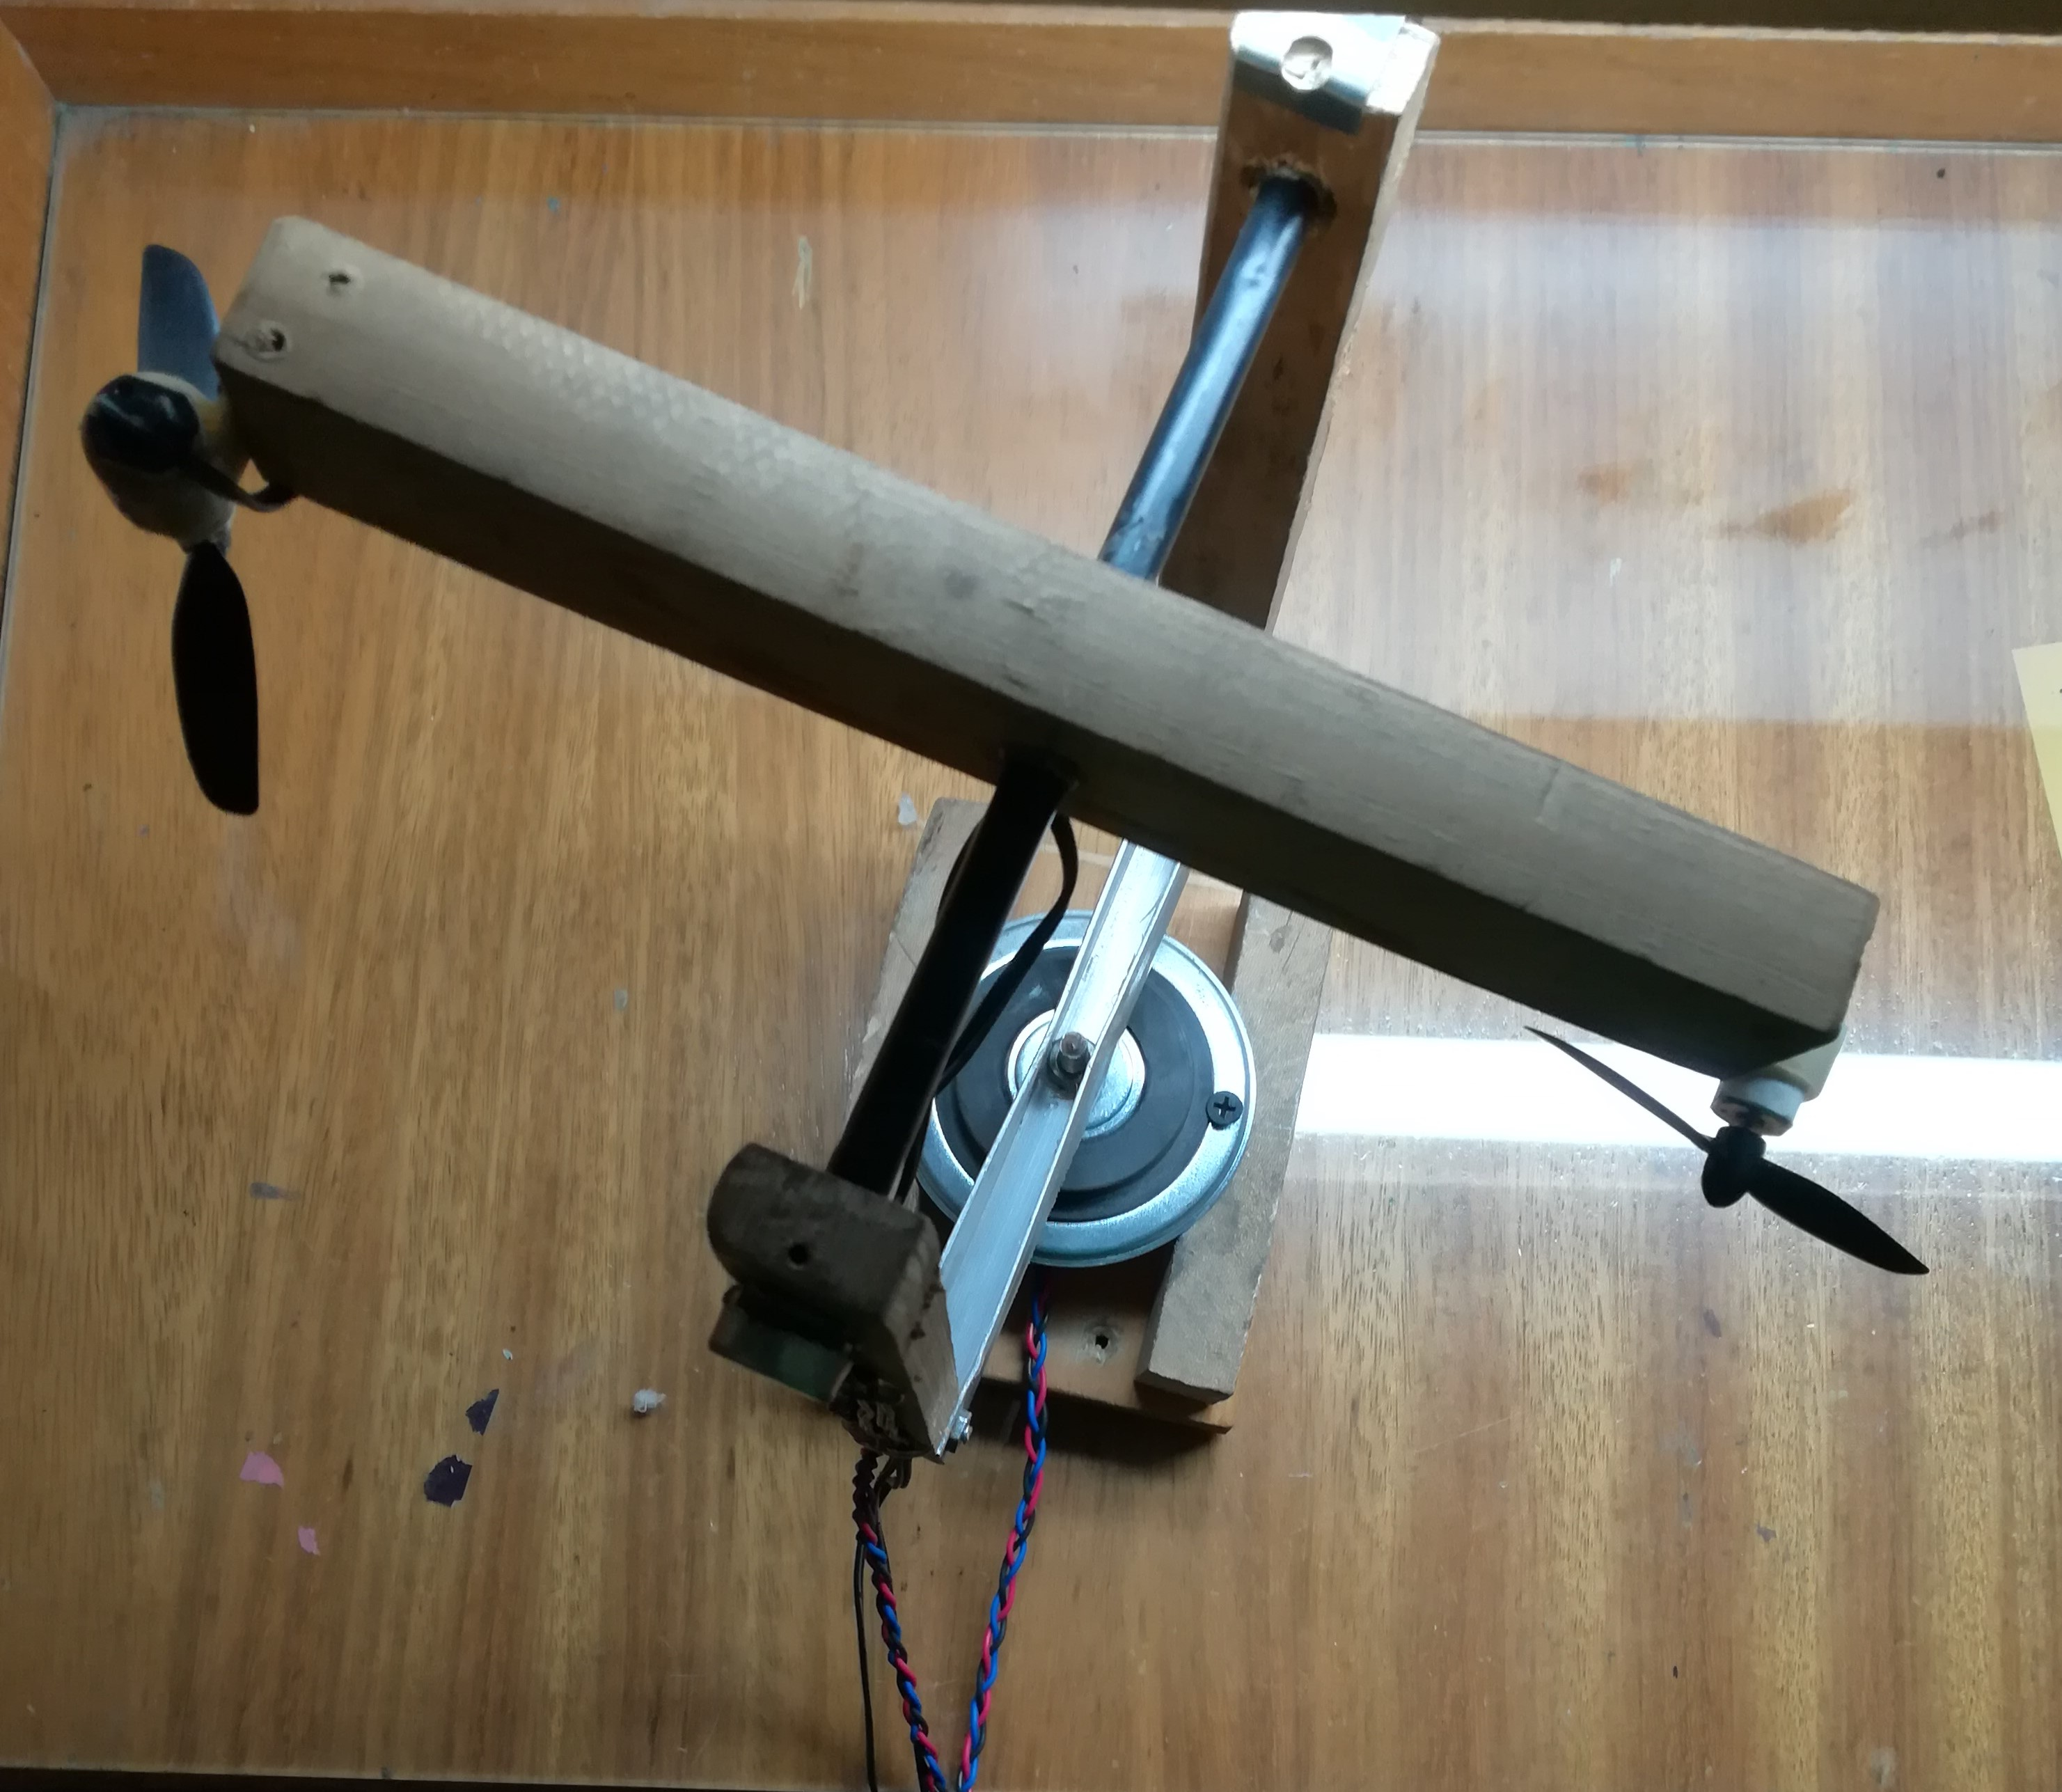
\includegraphics[width=0.7\linewidth]{images/modFinal2.jpg}
\caption{Simulador de sistema aerodinámico de helicóptero - Versión final}
\end{figure}

\newpage

\section{Análisis del sistema}
\subsection{Factores externos - Montaje}

Previo al planteo del sistema mecánico, se analizan los factores que afectarían al libre movimiento del mismo. Para dar el movimiento se incorporaron dos motores del estilo utilizado en drones, en este caso de hasta 25000 RPM.\\
La barra horizontal de madera sobre la que se montan ambos motores se la considera como una masa, la cual producirá una fuerza en oposición a la que traten de realizar los motores. Esto ya sea para el movimiento vertical (Pitch) u horizontal (Yaw). Para sujetar los motores se utilizaron dos bridas de plástico.\\
Por el centro de dicha barra de madera se hace pasar una barra de metal liviano, que actuará de eje vertical para que la barra de madera pueda rotar libremente.\\

\begin{figure}[H]
\centering
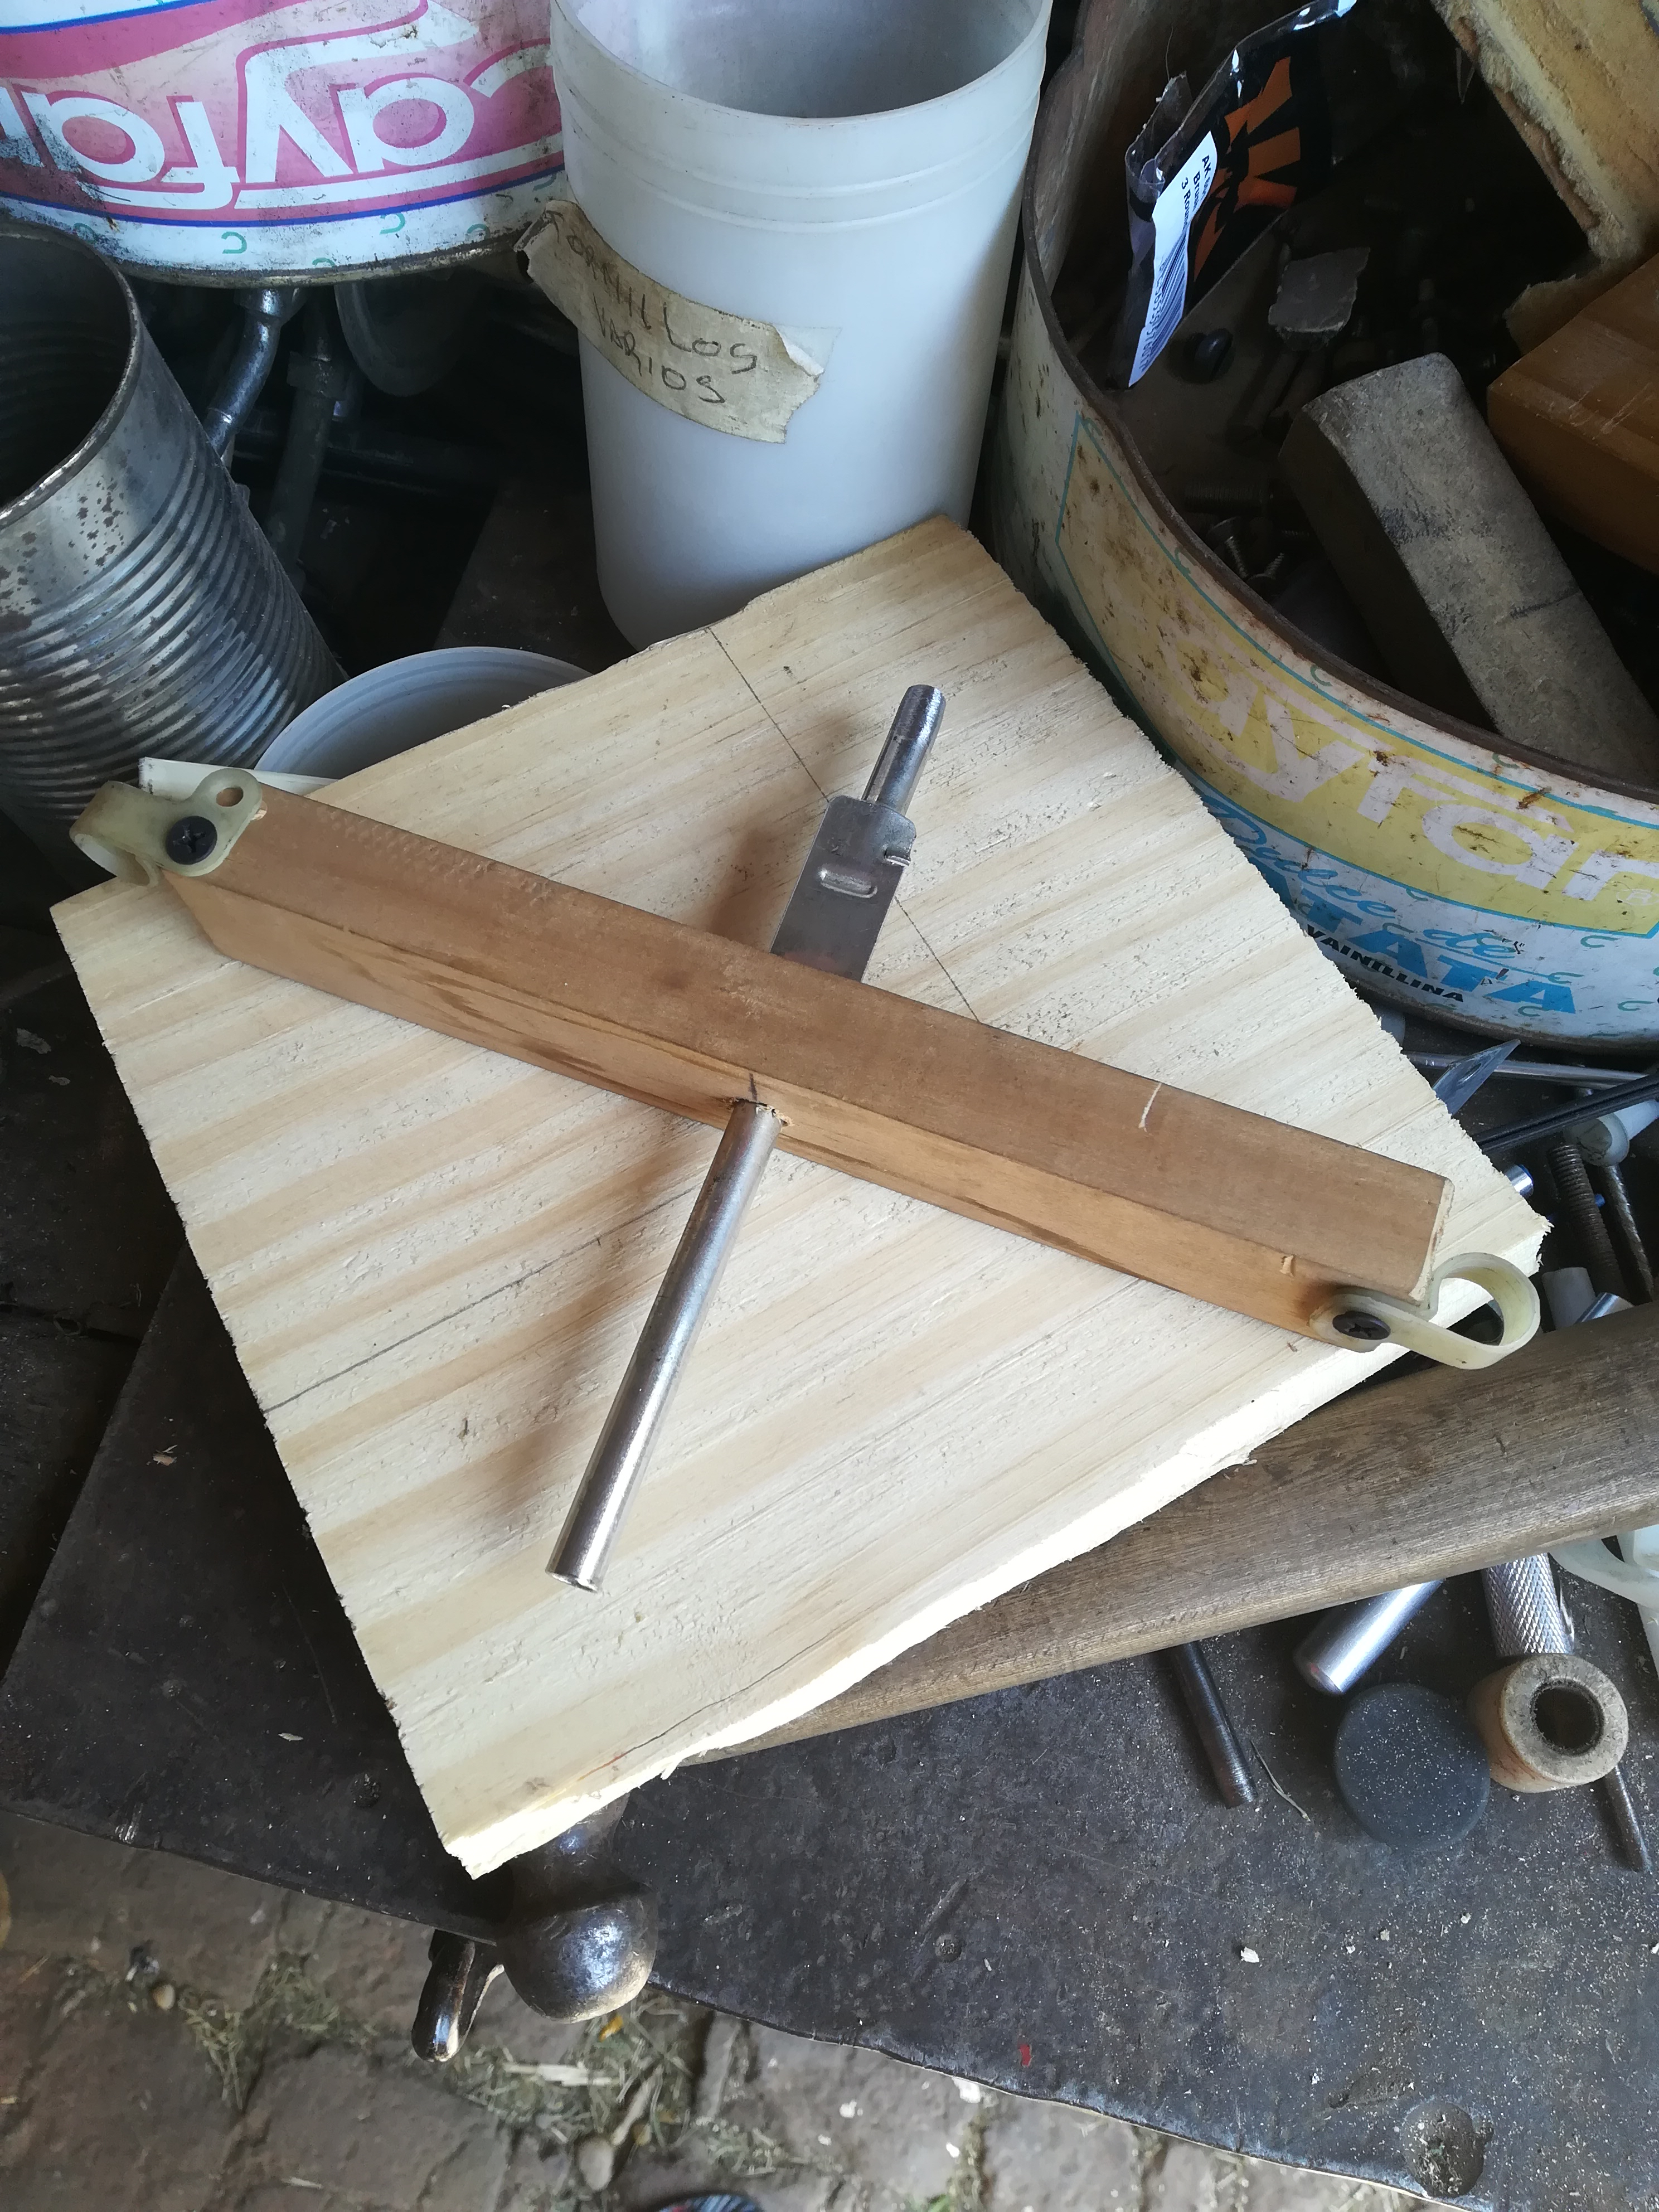
\includegraphics[width=0.4\linewidth]{images/rotor.jpg}
\caption{Barra de madera y eje}
\end{figure}

Esta barra de metal, en uno de sus extremos tiene colocado un potenciómetro (para poder tomar medición de la posición), y en el otro un ruleman para que el movimiento sea mas suave. Dicho ruleman se lo representará como un rozamiento vizcoso.\\
La barra de metal va colocada sobre sus extremos a un soporte en forma de 'U', sobre el cual van colocados el potenciómetro y ruleman mencionados previamente. El soporte en forma de 'U' está realizado sus laterales en madera, y la base sobre un perfil de aluminio. Esta pieza se la modelará como una masa.\\ En su centro, se colocó una pieza de ajuste para poder, mediante un tornillo y tuerca, unirlos a otro ruleman en la parte inferior, para dar un movimiento horizontal suave.\\

\begin{figure}[H]
\centering
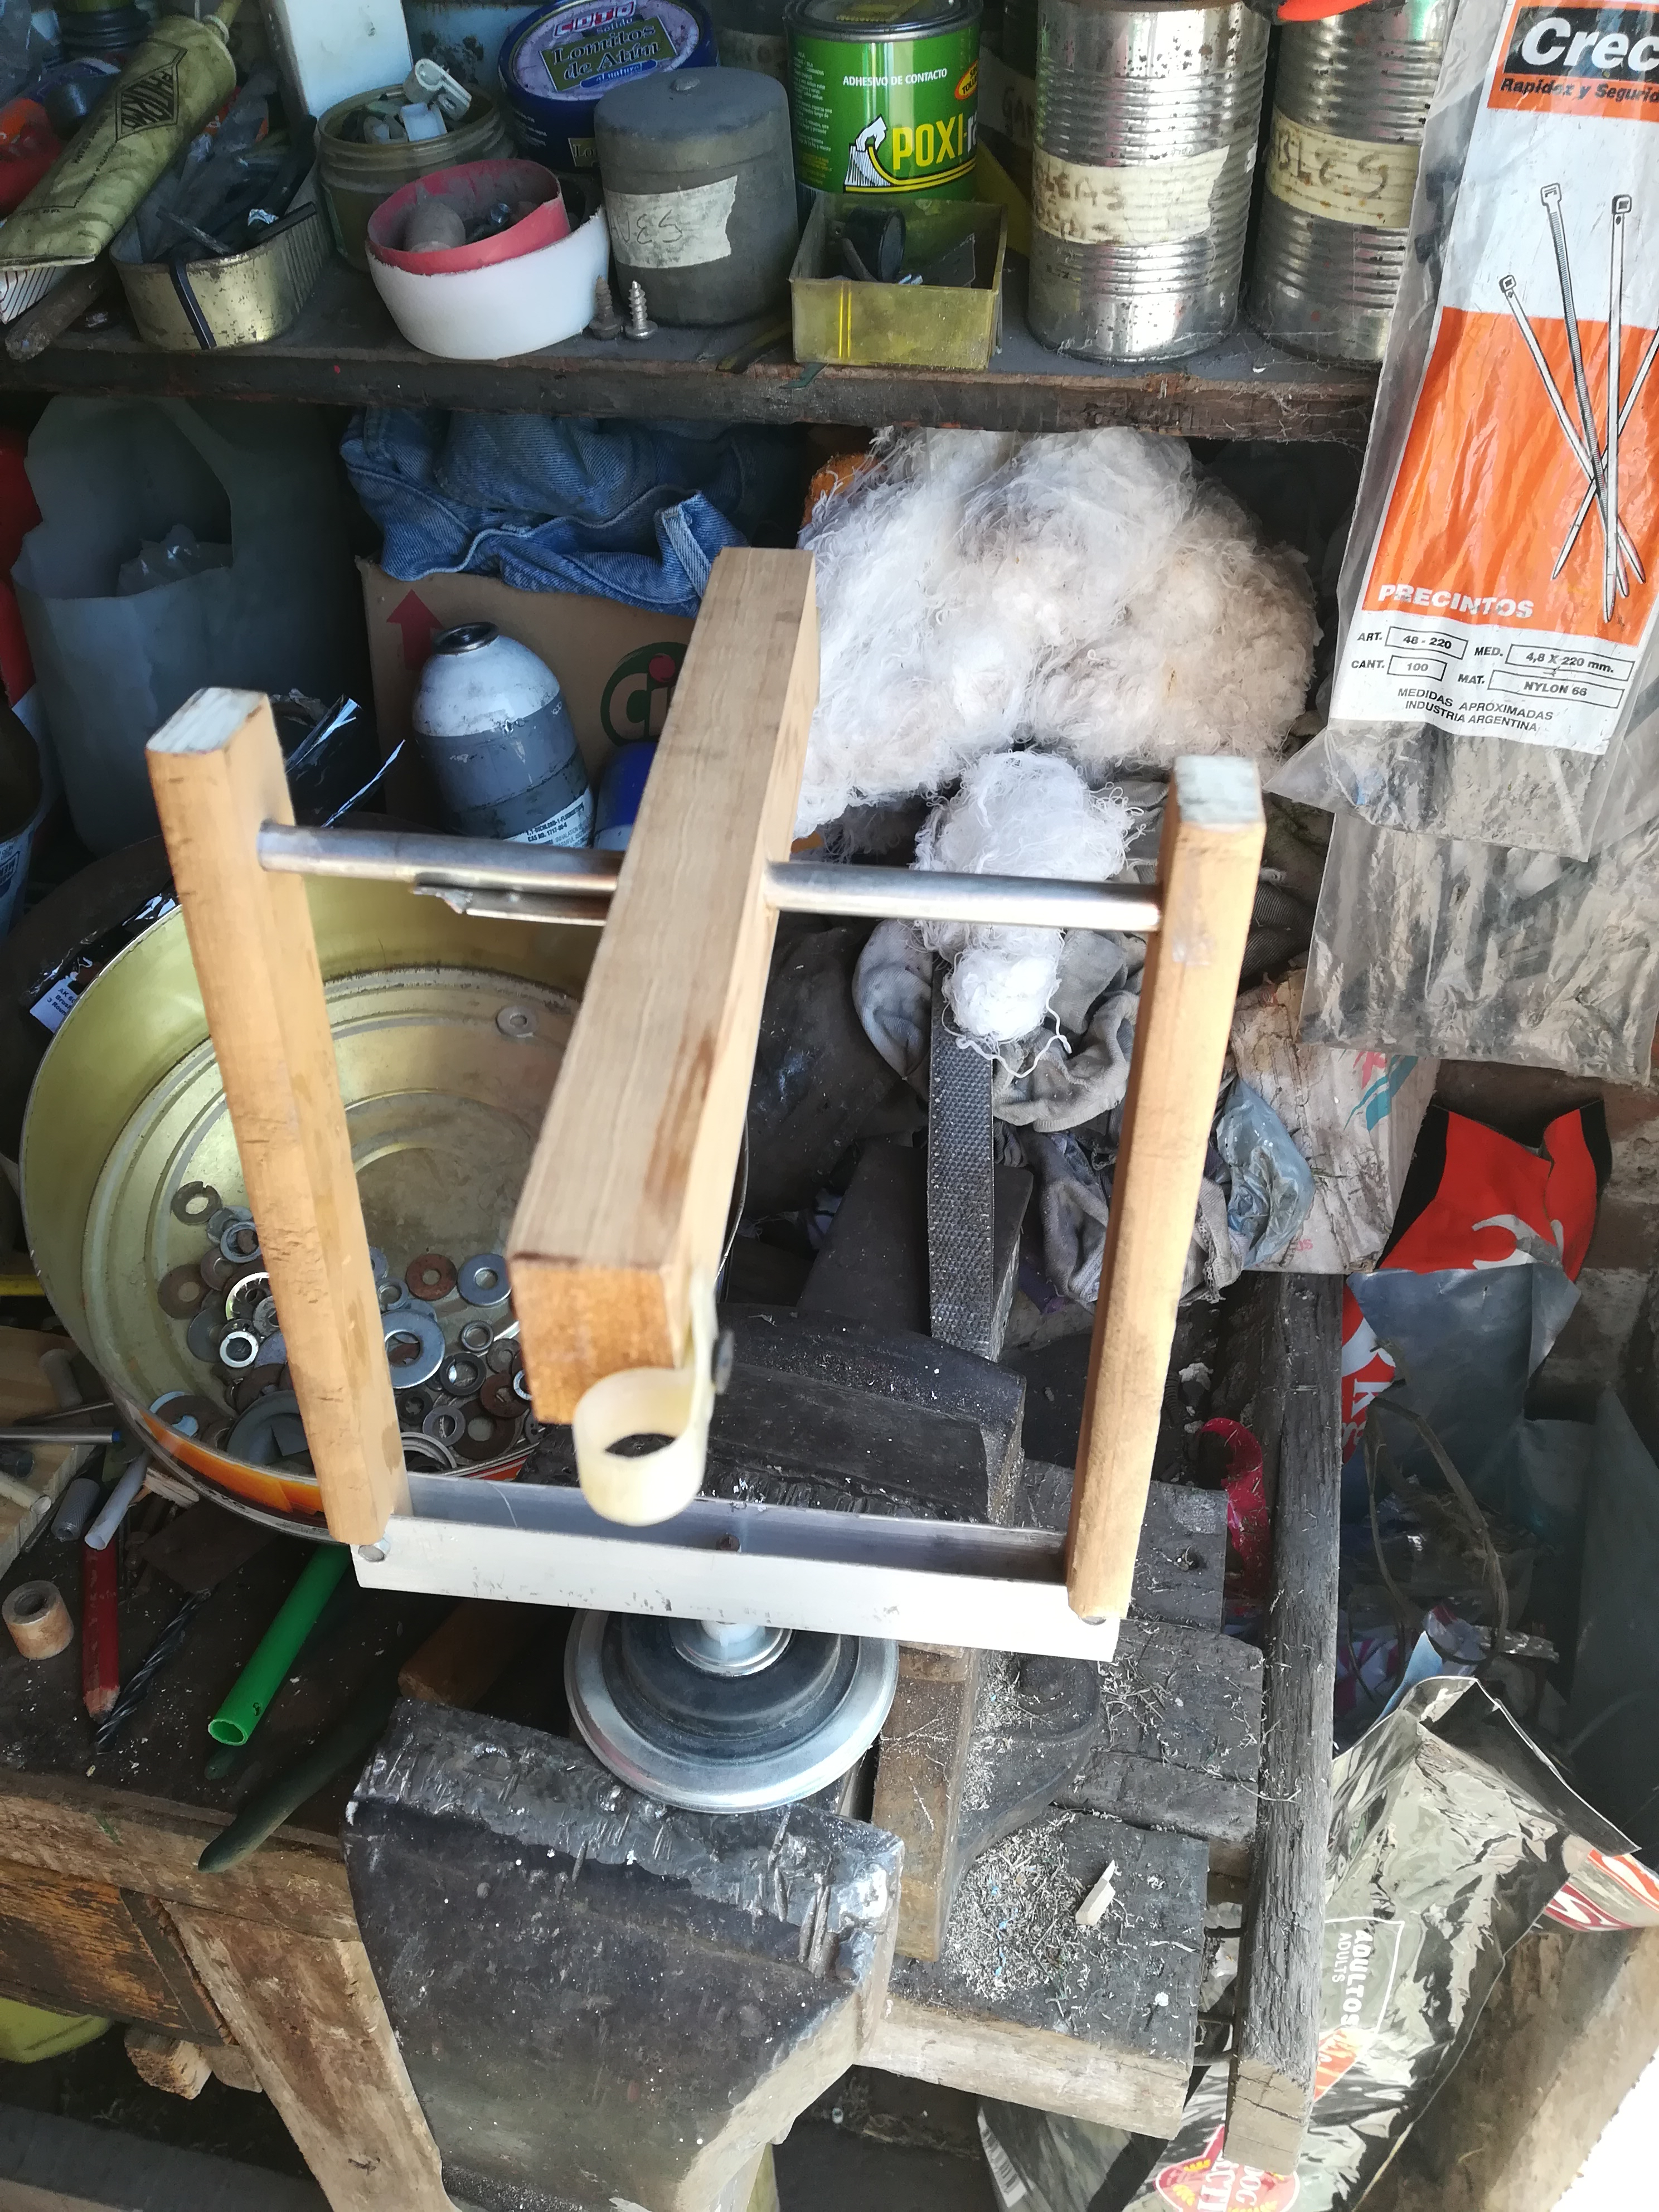
\includegraphics[width=0.4\linewidth]{images/preMontaje.jpg}
\caption{Modelo semiterminado}
\end{figure}

Finalmente, debajo de dicha pieza, adosado al tornillo se colocó otro potenciómetro, para poder medir el movimiento horizontal. 

\begin{figure}[H]
\centering
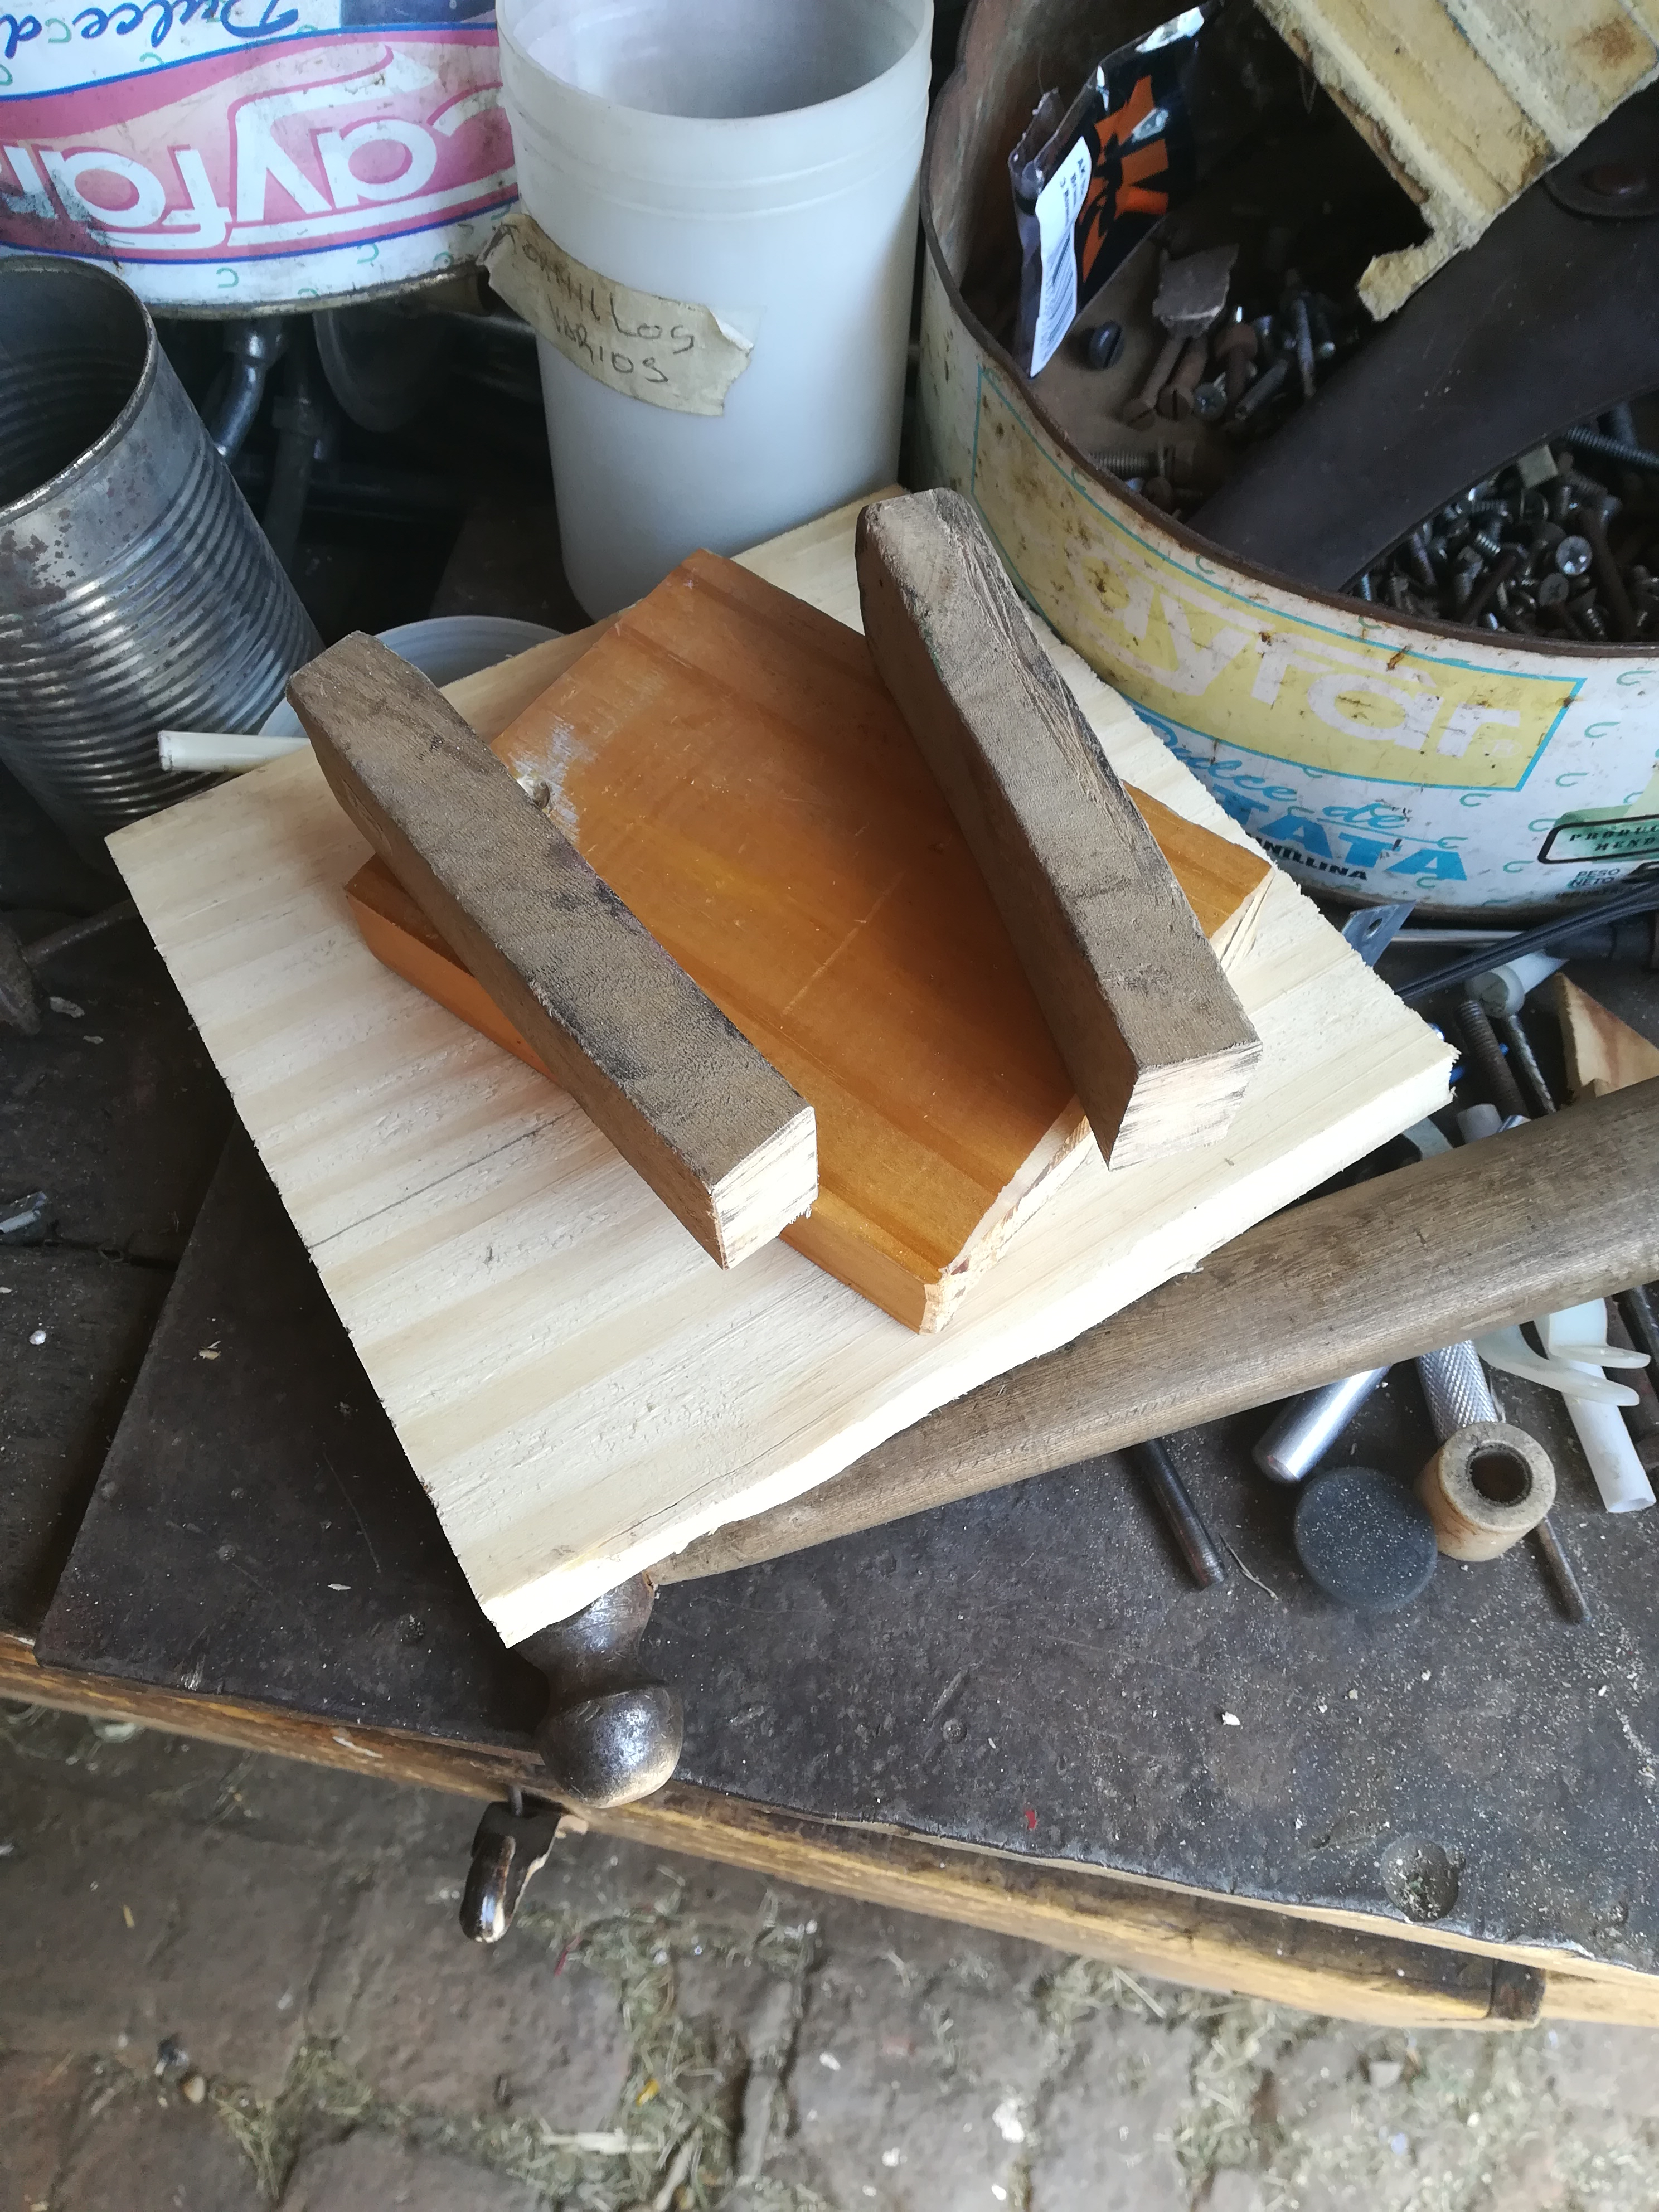
\includegraphics[width=0.4\linewidth]{images/base.jpg}
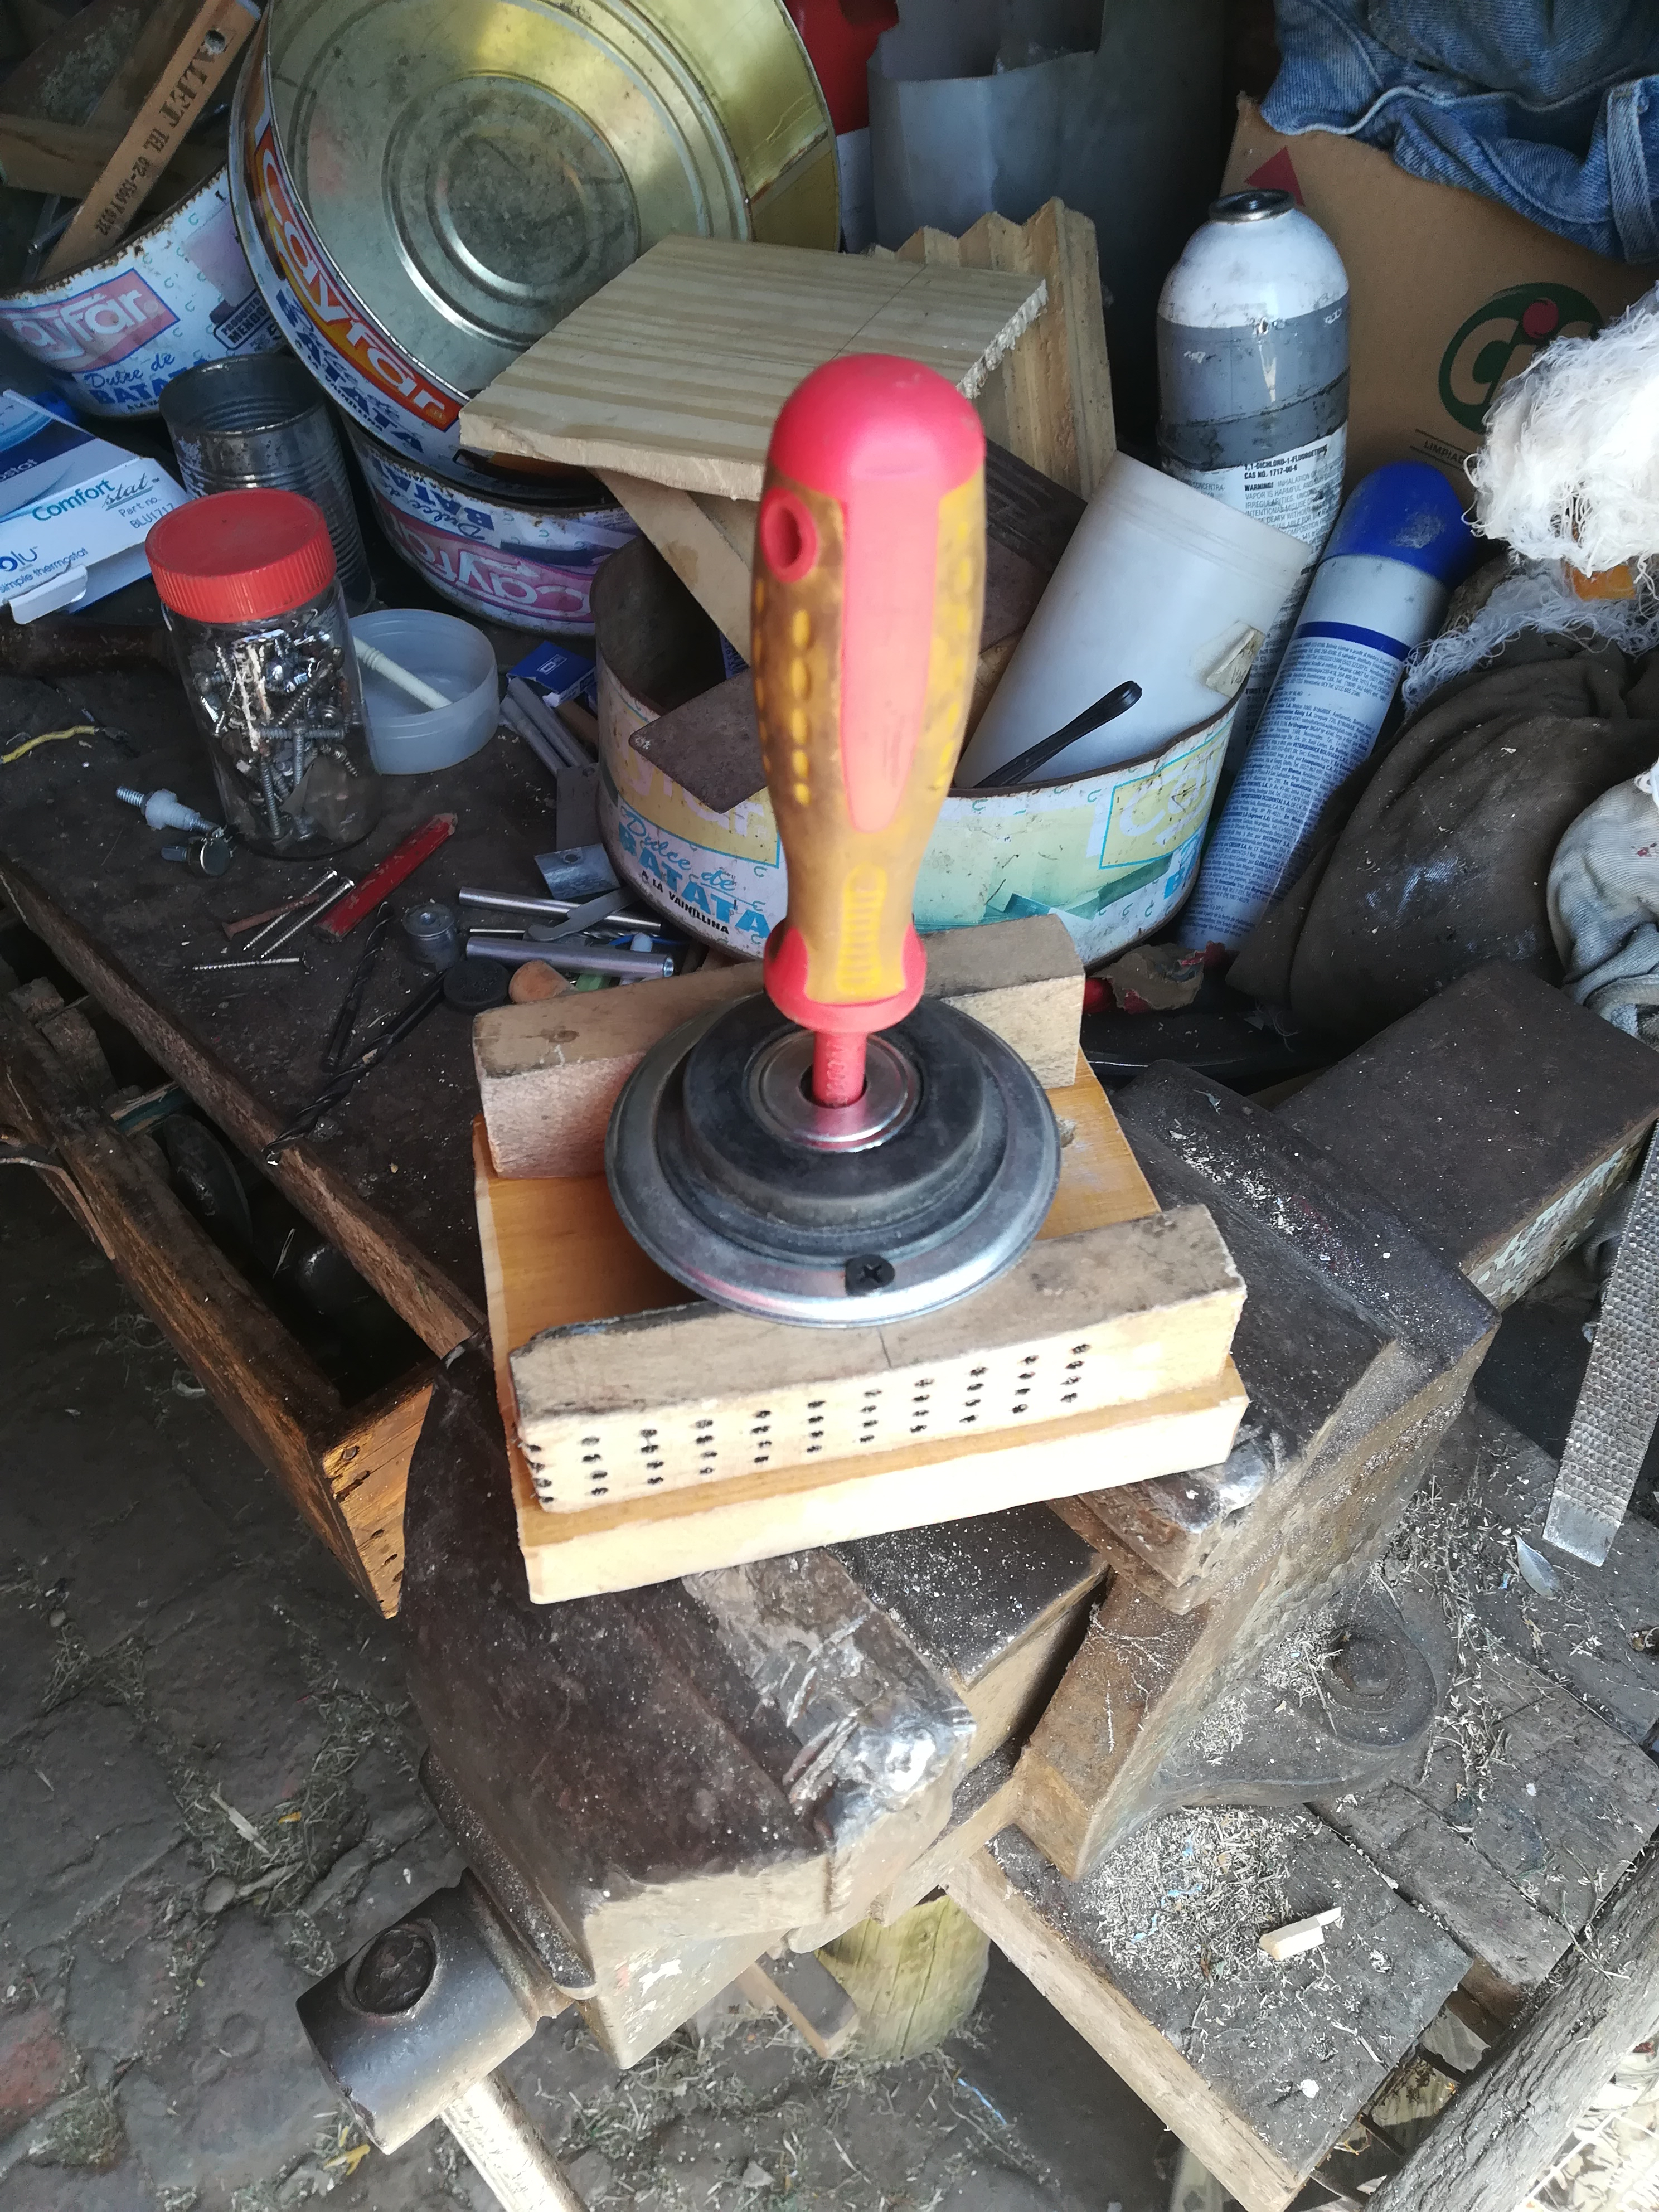
\includegraphics[width=0.4\linewidth]{images/baseU.jpg}\caption{Base y pieza de ajuste}
\end{figure}

\begin{figure}[H]
\centering
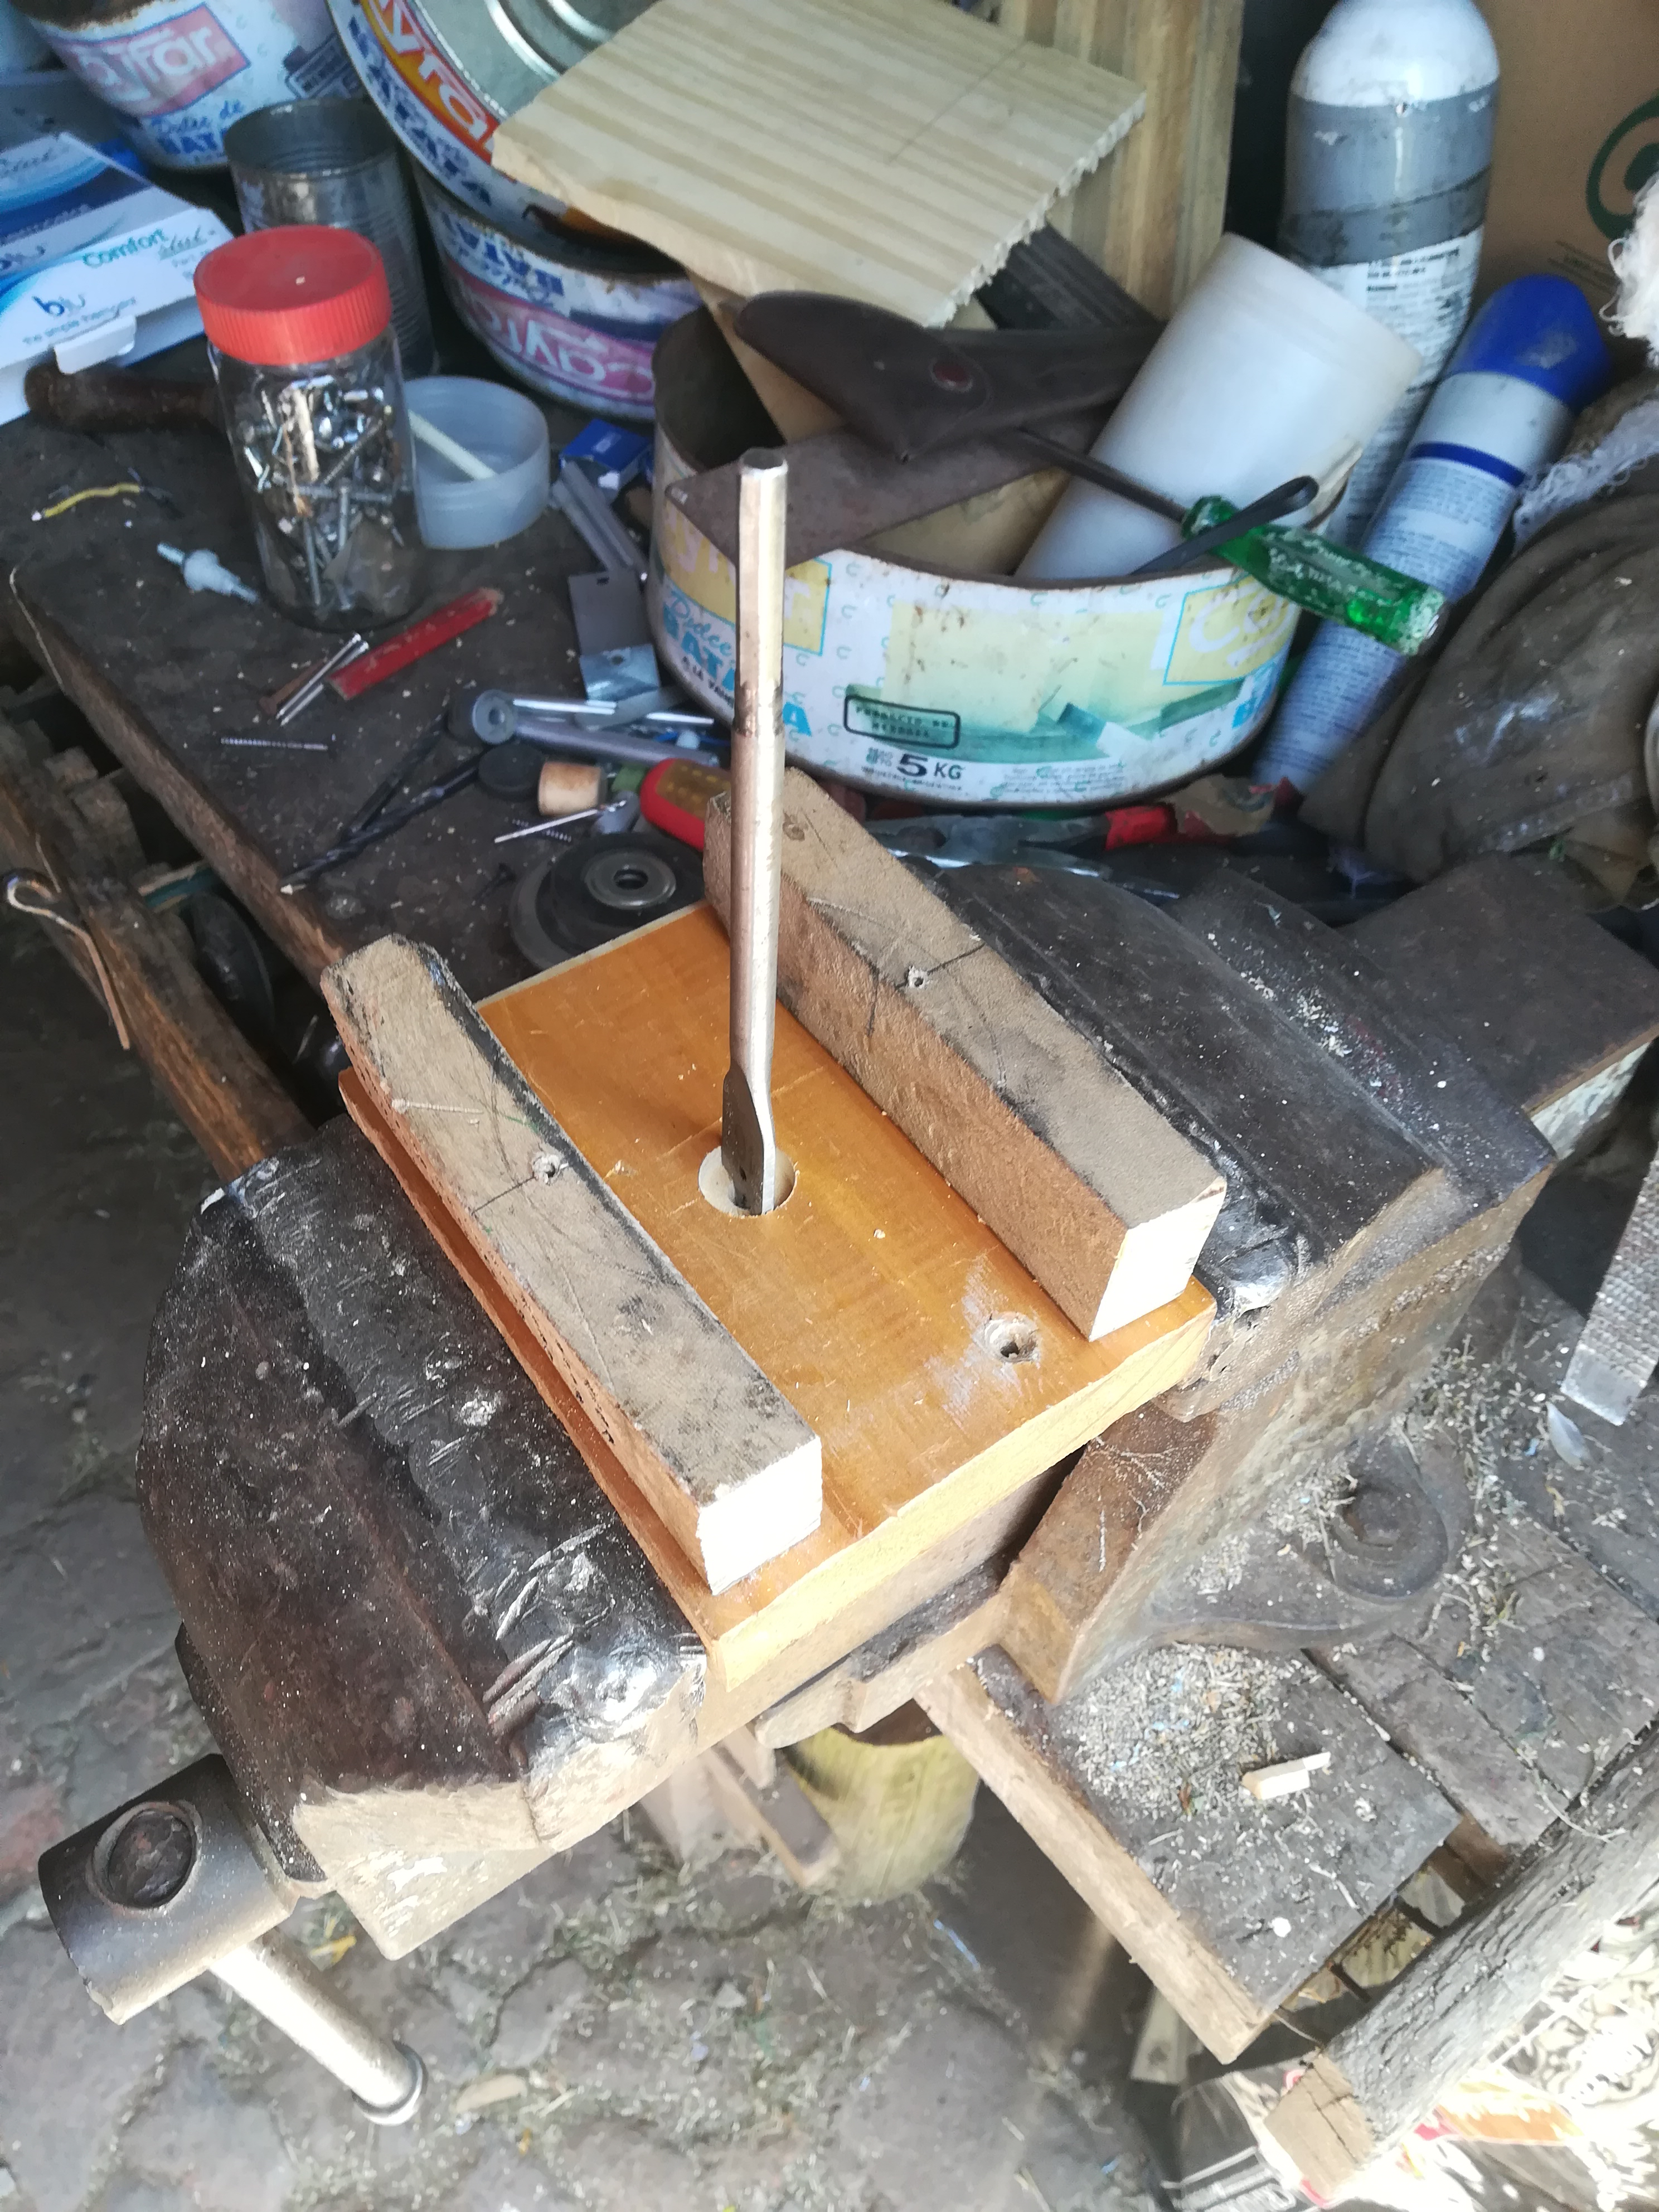
\includegraphics[width=0.4\linewidth]{images/poteBase1.jpg}
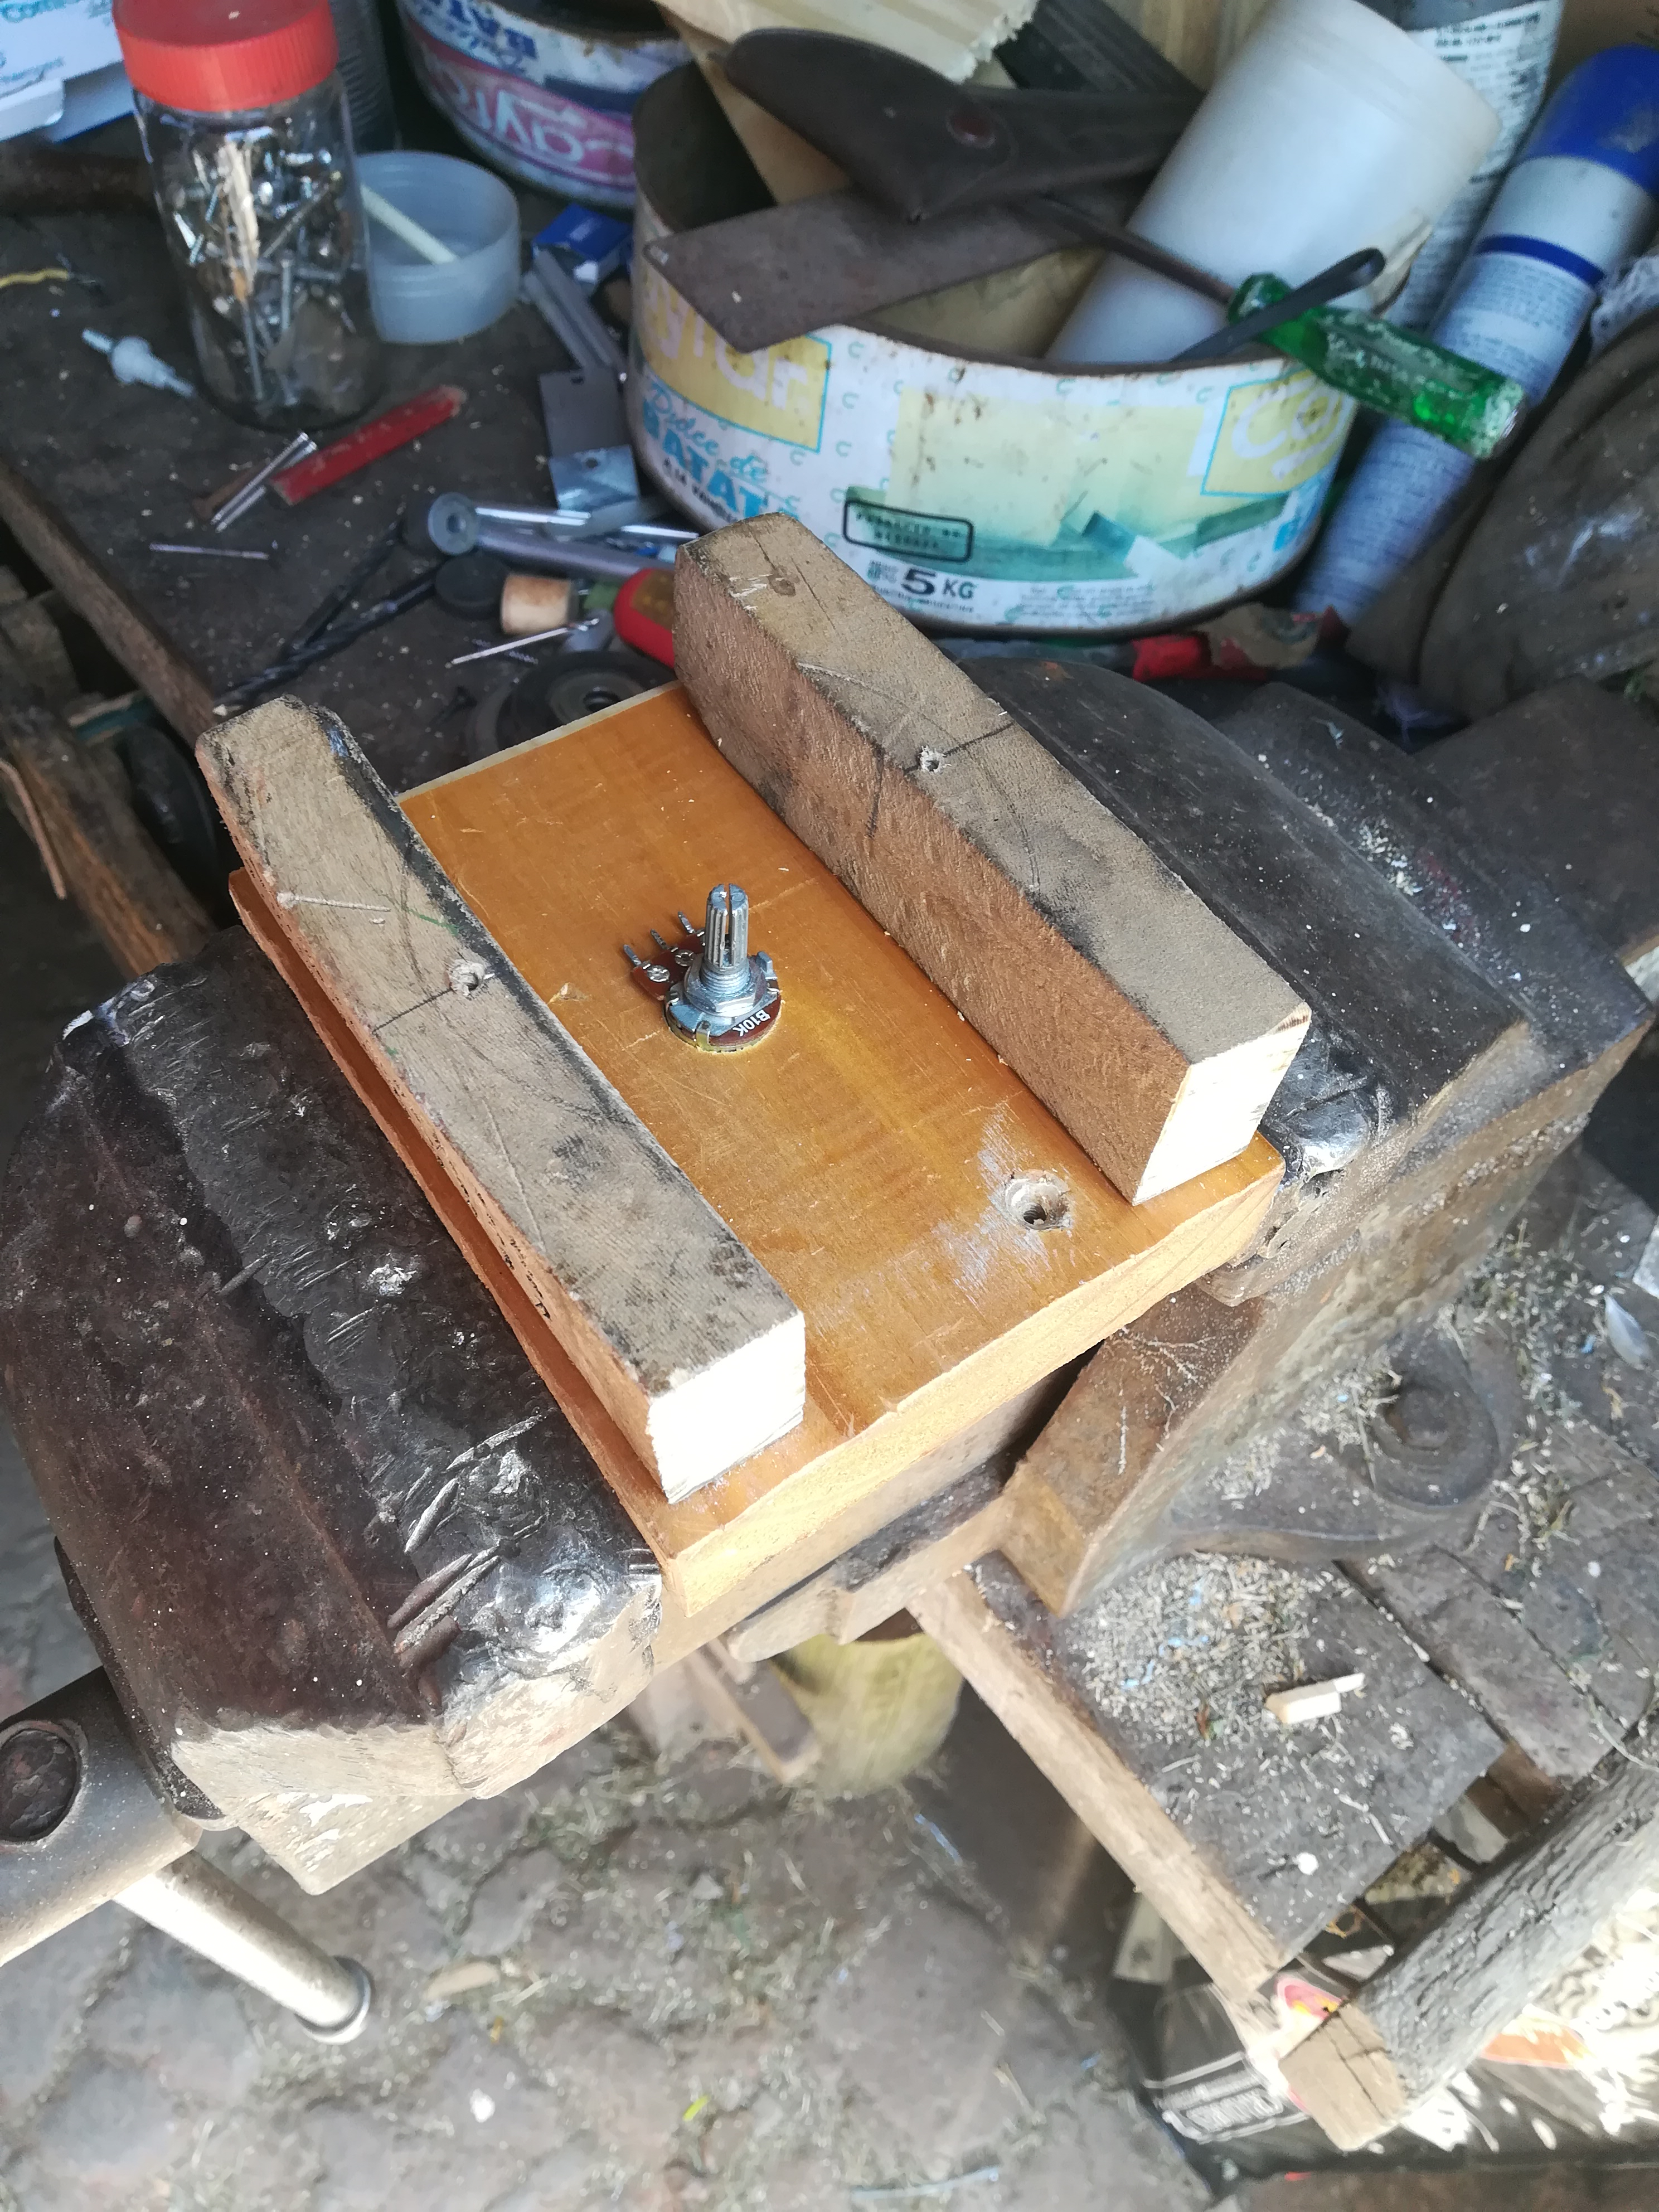
\includegraphics[width=0.4\linewidth]{images/poteBase2.jpg}\caption{Base agujereada y potenciómetro colocado}
\end{figure}

El conjunto queda apoyado sobre una base de madera, ajustando la pieza circular de ajuste con dos tornillos.

\begin{figure}[H]
\centering
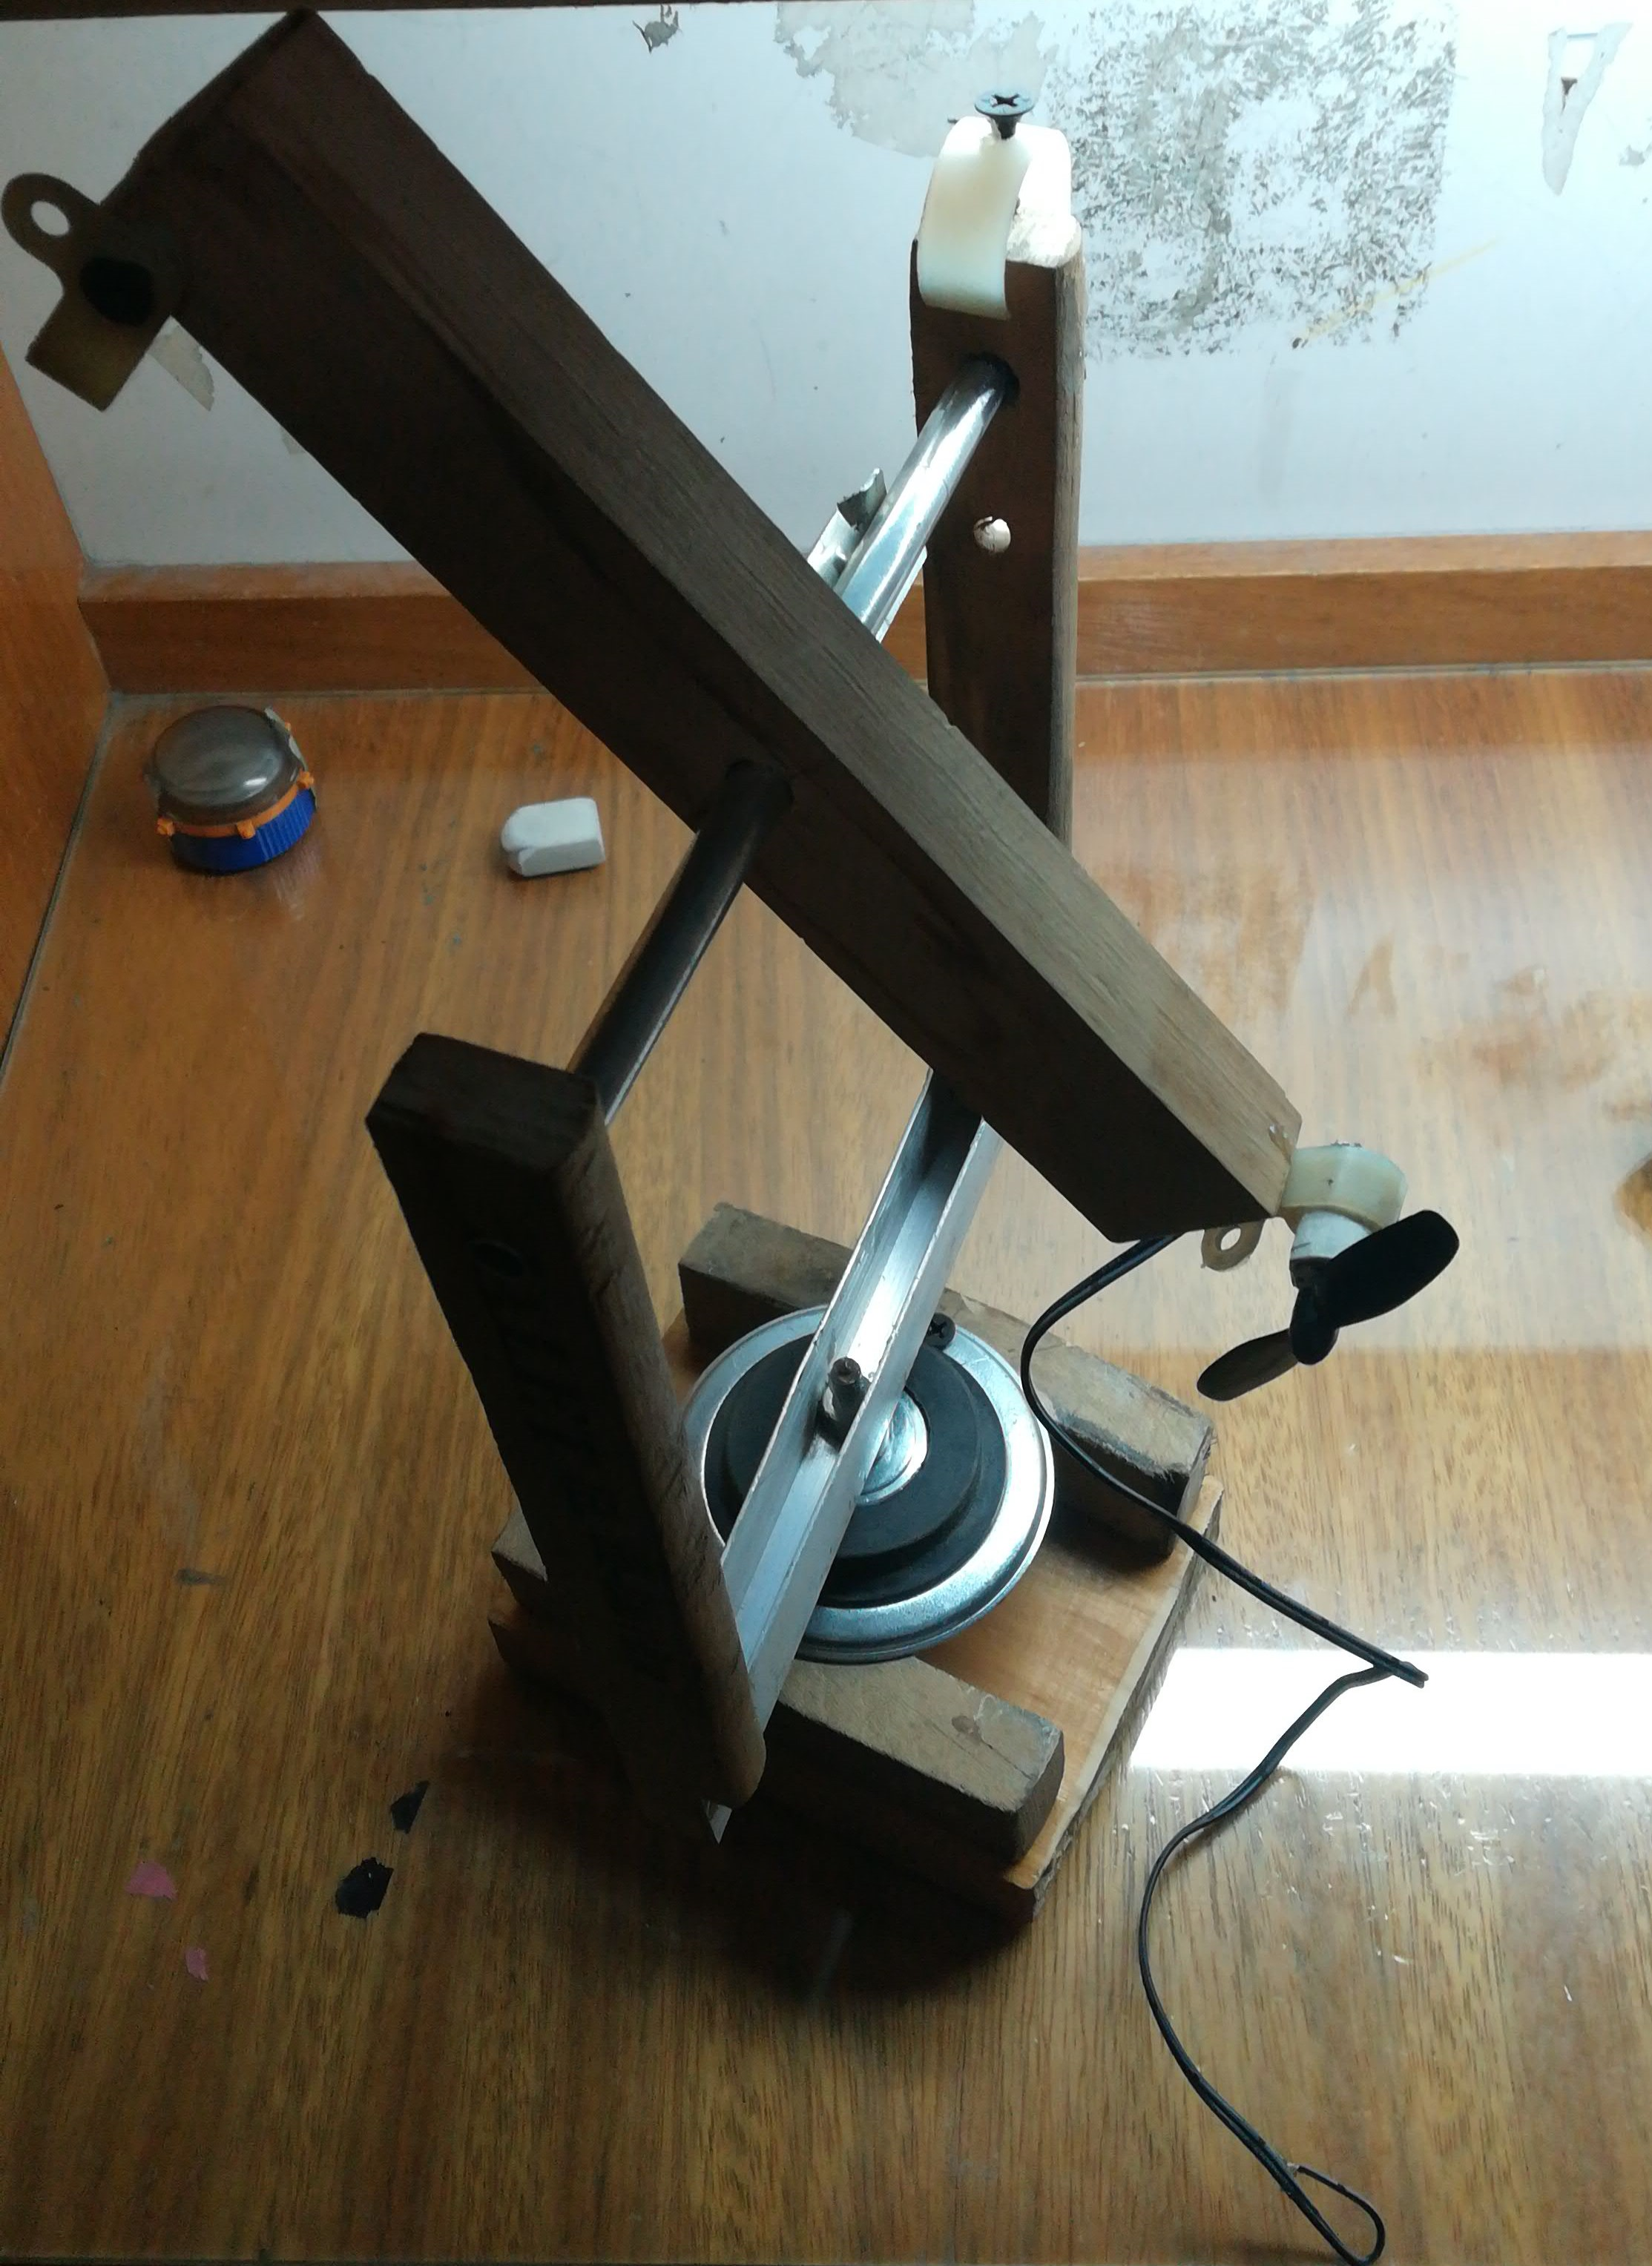
\includegraphics[width=0.4\linewidth]{images/modPrevio.jpeg}
\caption{Modelo terminado}
\end{figure}

\subsection{Sistema mecánico}
Teniendo los factores constructivos previamente mencionados, se realiza el siguiente modelo mecánico:

PONER FOTO, HACER DIBUJO

Notar que la particularidad de este sistema, es que posee dos variables de salida a controlar (cada una con uno de los potenciómetros). Planteando las ecuaciones físicas:

PONER ECUACIONES

Se acomodan las variables de interés, de manera de obtener el espacio de estados matricial:

PONER ESPACIO DE ESTADOS Y SI PUEDO LAS ECUACIONES ACOMODADAS 

\newpage

\section{Implementación en Arduino}
// aca es el codigo y como medimos las cosas, explicar tambien lo del puente H, que es un l298 hacia falta por la corriente y demas

\newpage

\section{Placa de interconexionado}

Para facilitar el conexionado al Arduino, se realizó una placa que actúa de interfaz entre este y el resto del sistema. Sobre ella se facilitan los siguientes elementos:

\begin{itemize}
\item Dos potenciómetros para poder realizar por un lado un control manual del Pitch, y por otro del Yaw.
\item Un conector polarizado para el potenciómetro que mide Pitch, y otro para el que mide Yaw.
\item Un conector polarizado para ingresar una señal externa para ajustar el Pitch, y otro para la señal de Yaw (más un jumper para puentearlas si se desea tener la misma señal para ambos).
\item Dos puntos de prueba para medir los valores de los potenciómetros con el osciloscopio.
\item Un conector polarizado para ingresar con la fuente externa para el Puente H.
\item Conectores polarizados para conectar los motores desde ésta placa hacia el Puente H.
\item Conectores polarizados para conectar las señales de control (PWM y las dos que determinan el sentido de giro) desde ésta placa hacia el Puente H.
\end{itemize}

\begin{figure}[H]
\centering
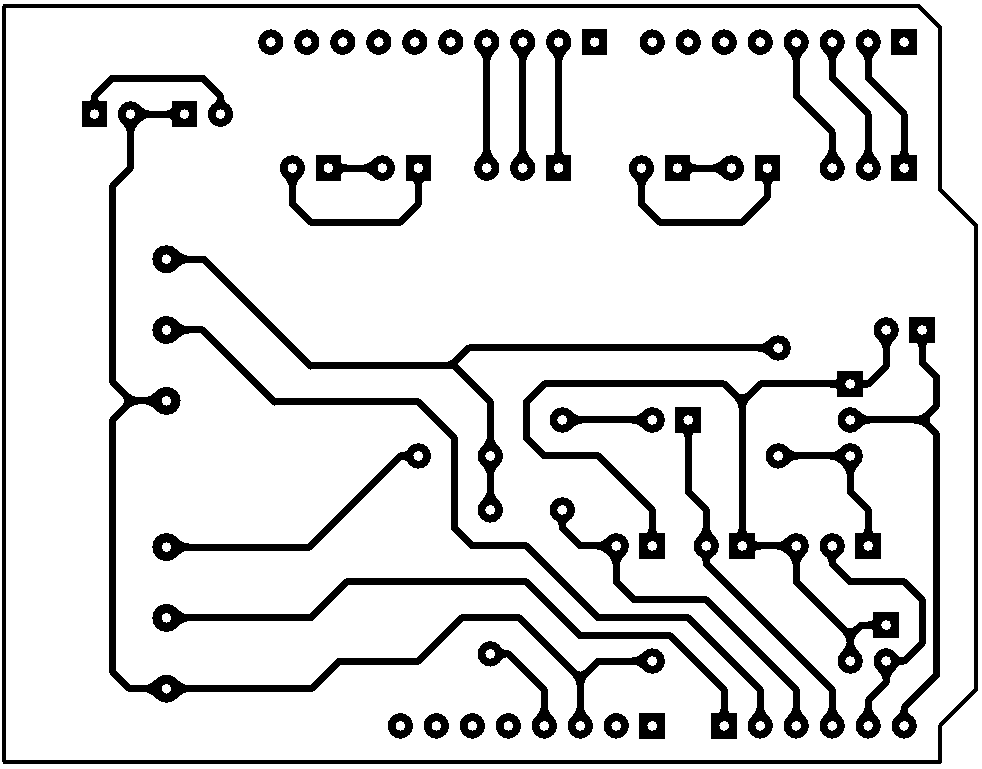
\includegraphics[width=0.4\linewidth]{images/cobre.png}
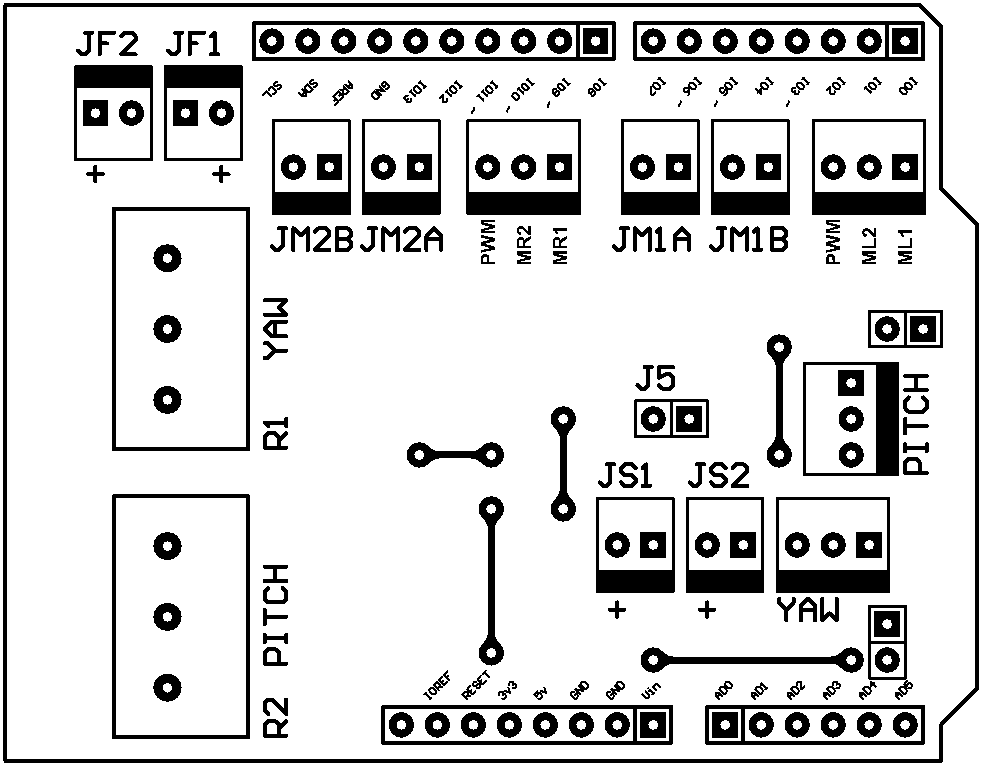
\includegraphics[width=0.4\linewidth]{images/componentes.png}\caption{PCB - Lado Cobre y Componentes}
\end{figure}

\newpage

\section{Mediciones}



\newpage

\section{Conclusiones}

los factores de inercia y roce son los que mas afectaron, y los cables que frenaban tambien, lo de las helices tambien, mejoras que se podrian hacer, motores mas potentes

\newpage

\section{Bibliografía}
\begin{itemize}
\item Idea para la maqueta: https://www.quanser.com/products/quanser-aero/
\item Funcionamiente básico y conexiones de la placa Puente H: https://www.prometec.net/l298n/ 
\item Motores con hélices: https://monarcaelectronica.com.ar/productos/motor-con-helice-12x20mm-dc-37v-25000rpm-mona/
\end{itemize}
\end{document}
